Resolution studies are used to quantify the precision of a timing reconstruction method.
The time resolution is determined from the difference between the reconstructed times of two hits (rechits) that are expected to be produced simultaneously.
Two complementary methods are employed to select such pairs of rechits, as illustrated in Fig.~\ref{trm_local_global_xstal}.

The first method selects a pair of adjacent crystals with similar energies within a single electromagnetic (EG) candidate cluster and is used to measure a \emph{local resolution}.
This approach probes the intrinsic single-crystal timing performance and provides sensitivity to delays arising from the readout electronics.
The second method selects a pair of rechits associated with electrons from a reconstructed $Z \rightarrow e^{+}e^{-}$ decay.
This \emph{global resolution} reflects the timing performance relevant for physics analyses, where hits originate from spatially separated regions of the detector.

\begin{figure}[htbp]
\begin{center}
\resizebox{0.7\textwidth}{!}{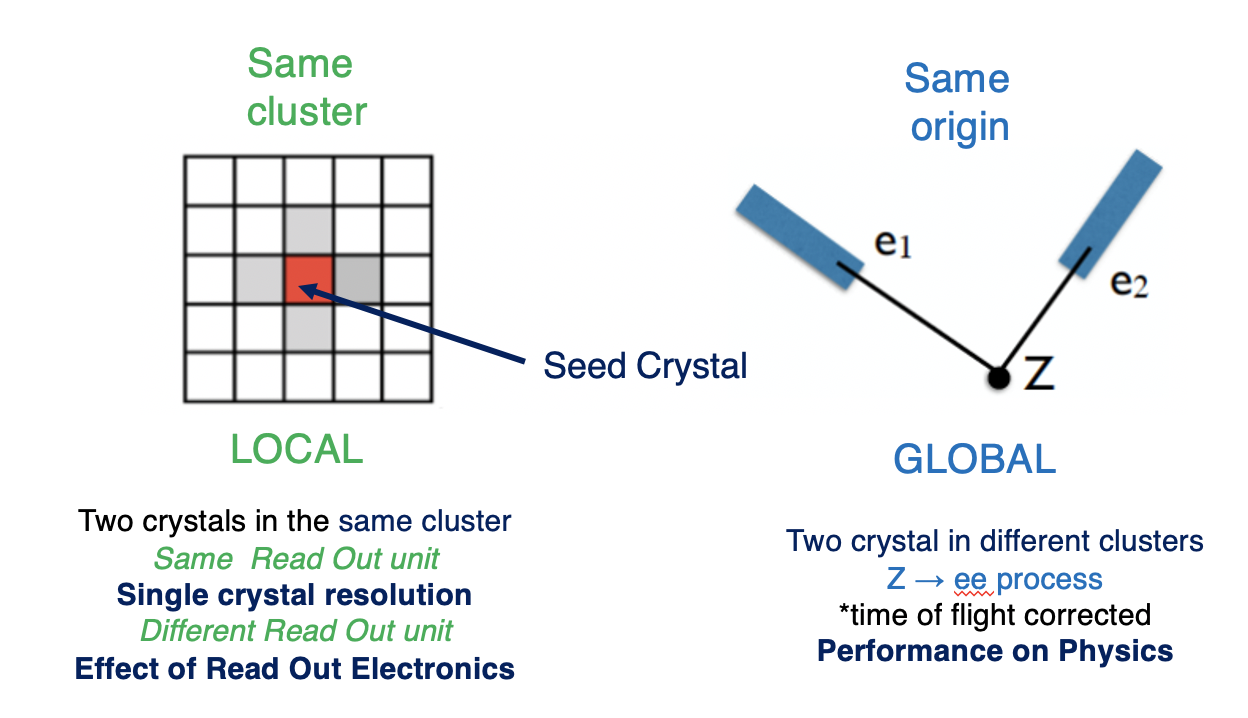
\includegraphics{fig/sec_method/Local_global_crystals.png}}
\caption{Methods used to select crystal pairs for time resolution measurements.
For the local resolution (right), two adjacent crystals within the same cluster are selected.
For the global resolution (left), seed crystals from two clusters associated with electrons from a $Z \rightarrow e^{+}e^{-}$ decay are used.}
\label{trm_local_global_xstal}
\end{center}
\end{figure}

For the local resolution, a pair of rechits is selected from the crystal cluster forming an EG candidate.
One crystal is required to be the seed crystal of the cluster, while the second must be an adjacent crystal in either the $\eta$ or $\phi$ direction.
The energy of the adjacent crystal is required to be within 20\,\% of the seed-crystal energy.
The EG candidate is further required to satisfy shower-shape criteria, with the semi-minor axis of the second moment of the cluster geometry satisfying $\texttt{smin} < 0.3$ and the semi-major axis satisfying $\texttt{smaj} < 0.5$.
If multiple EG candidates in an event satisfy these criteria, the candidate with the largest momentum is selected.

Local resolutions are further categorized based on whether the two crystals share the same readout electronics.
If both crystals are located within the same trigger tower, the measurement is referred to as a \emph{same readout unit} (\textbf{SRU}) resolution.
If the crystals are located in adjacent trigger towers, the measurement is referred to as a \emph{different readout unit} (\textbf{DRU}) resolution.
These local resolution categories probe both intrinsic detector timing performance and effects arising from readout electronics and pileup.

For the global resolution, seed crystals from two EG candidates matched to electrons from a $Z \rightarrow e^{+}e^{-}$ decay are selected.
Each EG candidate is required to be matched to an electron with $\Delta R < 0.1$, and the electron track $z$ position must be within 0.05\,cm of the primary-vertex $z$ position.
Pairs of EG candidates with an invariant mass between 60 and 150\,GeV are considered, and if multiple qualifying pairs are present, the pair with invariant mass closest to the nominal $Z$ boson mass is selected.

For the global resolution, a correction is applied to account for the difference in time-of-flight (TOF) of the two electrons from the primary vertex to their respective seed-crystal positions.
The resulting measurement is referred to as the \emph{$Z \rightarrow e^{+}e^{-}$} (\textbf{ZEE}) resolution.
The selection criteria used for the SRU, DRU, and ZEE resolution measurements are summarized in Table~\ref{res_params}.

As illustrated in Fig.~\ref{trm_timeproccess}, the time difference between the two selected rechits,
$\Delta(\text{Seed Time}) = t_{1} - t_{2}$,
is evaluated as a function of an effective amplitude, $A_{\mathrm{eff}} / \sigma_{N}$, which is proportional to the energy of the corresponding EG candidates.
The effective amplitude is defined as
\begin{equation}
A_{\mathrm{eff}}/\sigma_{N} =
\frac{(A_{1}/\sigma_{N_{1}})(A_{2}/\sigma_{N_{2}})}
{\sqrt{(A_{1}/\sigma_{N_{1}})^{2} + (A_{2}/\sigma_{N_{2}})^{2}}} \, ,
\label{eq_a}
\end{equation}
where $A_{i}$ is the pulse amplitude measured in crystal $i$ and $\sigma_{N_{i}}$ is the corresponding pedestal noise.

The distribution of $\Delta(\text{Seed Time})$ is formed in bins of $A_{\mathrm{eff}}/\sigma_{N}$ and fitted with a Gaussian function.
The standard deviation $\sigma(t_{1}-t_{2})$ extracted from each fit is then plotted as a function of the central value of the corresponding $A_{\mathrm{eff}}/\sigma_{N}$ bin.

\begin{figure}[htbp]
\begin{center}
\resizebox{0.95\textwidth}{!}{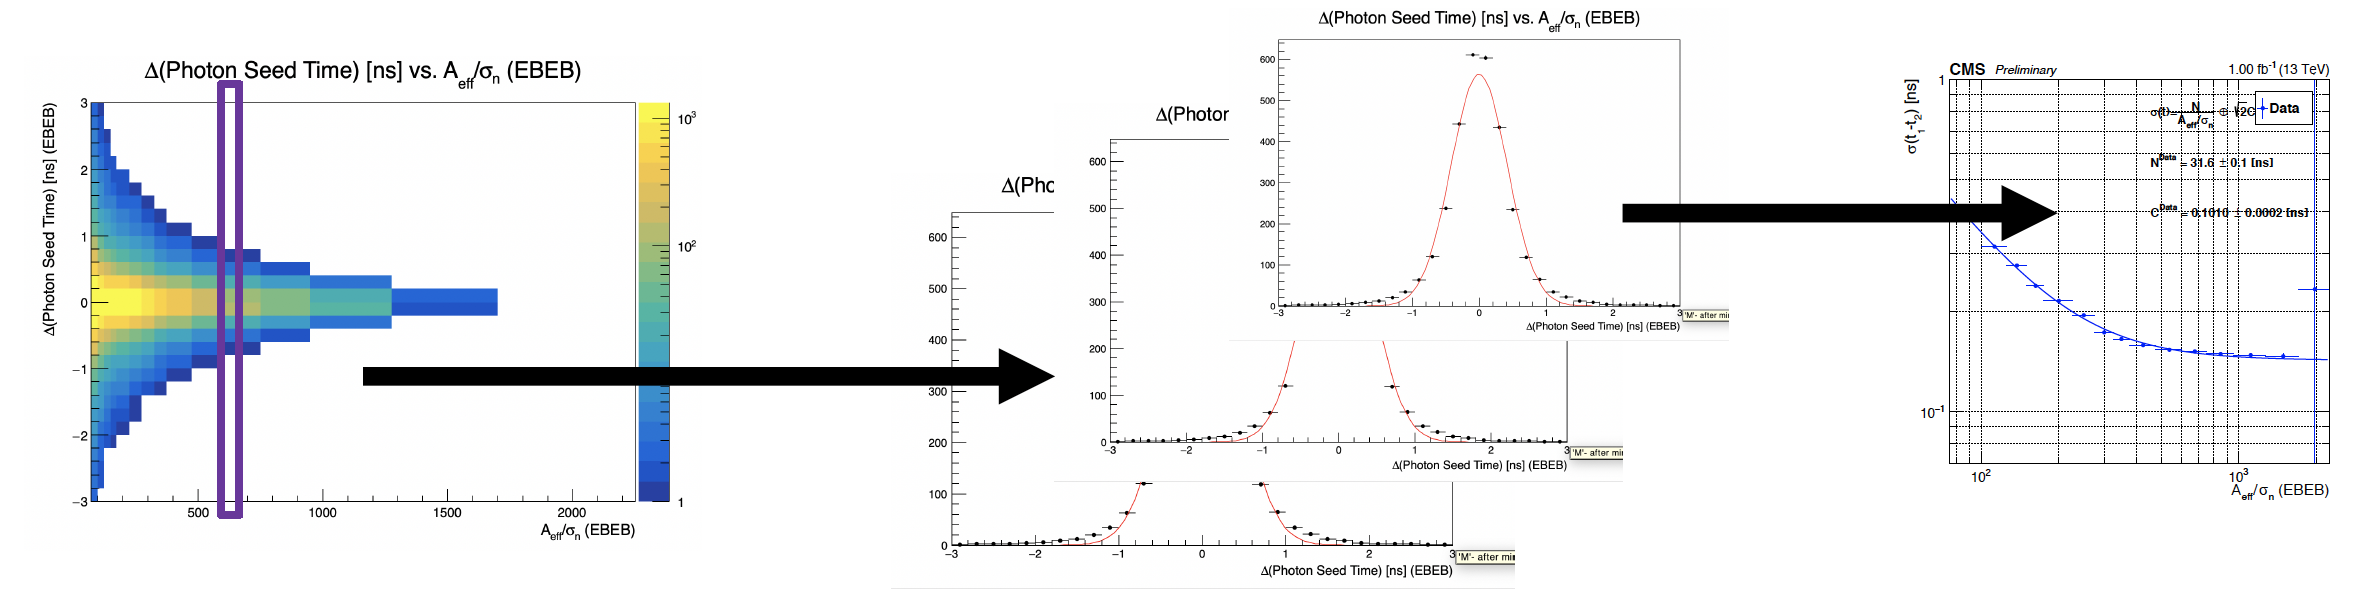
\includegraphics{fig/sec_method/timeres_process.png}}
\caption{Procedure used to extract the time resolution.
The distribution of $\Delta(\text{Seed Time})$ is formed in bins of $A_{\mathrm{eff}}/\sigma_{N}$ and fitted with a Gaussian.
The extracted standard deviation $\sigma(t_{1}-t_{2})$ is plotted as a function of $A_{\mathrm{eff}}/\sigma_{N}$ and fitted using the resolution parameterization described in the text.}
\label{trm_timeproccess}
\end{center}
\end{figure}

The dependence of $\sigma(t_{1}-t_{2})$ on $A_{\mathrm{eff}}/\sigma_{N}$ characterizes the time resolution and is traditionally described by
\begin{equation}
\sigma^{2}_{i} =
\left(\frac{N}{A_{\mathrm{eff}}/\sigma_{N}}\right)^{2} + 2C^{2} \, ,
\label{eq_b}
\end{equation}
where $N$ parameterizes the contribution from electronic noise and $C$ is a constant term.
The constant term includes contributions from variations in shower development within the crystal, crystal-to-crystal differences in pulse shapes, readout-unit-dependent delays, and pileup effects.
For each resolution category (SRU, DRU, and ZEE), the constant term $C$ represents the asymptotic timing resolution at high signal amplitude.

To better describe the resolution behavior at lower effective amplitudes, the parameterization can be extended to include a stochastic term,
\begin{equation}
\sigma^{2}_{i} =
\left(\frac{N}{A_{\mathrm{eff}}/\sigma_{N}}\right)^{2}
+ \frac{S^{2}}{A_{\mathrm{eff}}/\sigma_{N}}
+ 2C^{2} \, ,
\label{eq_c}
\end{equation}
where $S$ captures additional fluctuations that scale inversely with signal amplitude.
While this term is not traditionally included, its addition improves the quality of the fit when extending the analysis to lower values of $A_{\mathrm{eff}}/\sigma_{N}$.
This extended parameterization is used for resolution measurements performed with the CC timing reconstruction.

\hfill
\begin{table}[h!]
\begin{center}
 \begin{tabular}{ |c| }
 \hline
 Resolution Selection Cuts \\
 \hline
 \hline
 Local Resolution\\
 \hline
  %isOOT false \\
  %At least one photon candidate \\
  Photon smin $>$ 0.3 \\
  Photon smaj $>$ 0.5 \\
  %choose a seed crystal and an adjacent crystal to the seed crystal\\ 
  Photon seed crystal has an adjacent crystal where : \\ 
  seed crystal energy $<$ 120\% adjacent crystal energy \\
  Qualifying seed crystal with largest energy \\
 \hline
 Global Resolution\\
 \hline
  Photon has PixSeed \\
  Photon gedID $<$ 3 \\
  %isOOT false \\
  Photon matches to an electron with dR $<$ 0.1  \\
  Matching electron has trackZ within 1.0 cm of primary vertex Z \\
  At least 2 qualifying photons \\
  Pair of photons with combined mass $<$ 150 GeV \& $>$ 60 GeV \\
  Qualifying pair of photons with combined mass closets to Z mass \\
\hline
\end{tabular}
\end{center}
\caption{Selection cuts for local and global resolutions.}
\label{res_params}
\end{table}
